This layer is for communication between the control layer and the UR5 layer in details. It have a router as its subsystem. The router uses DHCP to allow IP addresses to be assigned to the UR5's control box and the Raspberry Pi.

\subsection{Network Layer Hardware}
N/A

\subsection{Network Layer Operating System}
N/A

\subsection{Netowrk Layer Software Dependencies}
Requires TCP/IP socket connection method in software.

\subsection{Router}
Router is the only piece of hardware in the Network Layer. It requires Ethernet cables to be connected to the UR5 control box and Raspberry Pi  establish  TCP/IP socket connection for issuing commands to the UR5's robotic arm.

\begin{figure}[h!]
	\centering
 	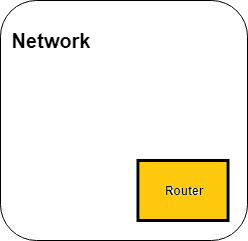
\includegraphics[width=0.60\textwidth]{images/Network_Layer_Router}
 \caption{Router Subsystem diagram}
\end{figure}

\subsubsection{Router Subsystem Hardware}
Standard wired Ethernet router.

\subsubsection{Router Subsystem Operating System}
N/A

\subsubsection{Router Subsystem Software Dependencies}
Requires TCP/IP socket connection method in software.

\subsubsection{Router Subsystem Programming Languages}
N/A

\subsubsection{Router Subsystem Data Structures}
Structure of commands issued from Raspberry Pi to UR5 are sent as strings converted to bytes. For example the string 'stop(1.0)' would be converted to bytes and sent to the robot to tell it to stop.

\subsubsection{Router Subsystem Data Processing}
N/A


